\documentclass[11pt,a4paper]{article}

% Compile with XeLaTeX from the paper directory.
\usepackage{fontspec}
\setmainfont{Times New Roman}
\usepackage[a4paper,top=2.2cm,bottom=2.2cm,left=2.5cm,right=2.5cm]{geometry}
\usepackage{microtype}
\usepackage{setspace}
\setstretch{1.12}
\usepackage{amsmath,amssymb}
\usepackage{booktabs}
\usepackage{graphicx}
\usepackage{float}
\usepackage{caption}
\usepackage{enumitem}
\usepackage{xcolor}
\usepackage{hyperref}
\usepackage{url}
\usepackage{indentfirst}
\usepackage{siunitx}

\hypersetup{
  colorlinks=true,
  linkcolor=black,
  citecolor=black,
  urlcolor=blue,
  pdftitle={Dự đoán cường độ carbon của ngành điện bằng Machine Learning sử dụng dữ liệu Our World in Data giai đoạn 2000--2025},
  pdfauthor={Nguyễn Thành Long, Nguyễn Đức Huy, Hồ Quốc Sử, Bùi Lê Thanh Ngân}
}
\captionsetup{font=small,labelfont=bf}
\setlength{\parindent}{1.2cm}
\setlength{\parskip}{0.25em}
\setlist[itemize]{topsep=0.3em,itemsep=0.2em}

% Auto-generated by src/carbon_intensity_workflow.py. Do not edit manually.
\newcommand{\DatasetRows}{5281}
\newcommand{\DatasetCountries}{212}
\newcommand{\TrainRows}{3944}
\newcommand{\ValidationRows}{632}
\newcommand{\TestRows}{705}
\newcommand{\ExcludedRows}{409}
\newcommand{\BestModel}{XGBoost}
\newcommand{\BestTestMAE}{24.25}
\newcommand{\BestTestRMSE}{41.03}
\newcommand{\BestTestRSquared}{0.972}
\newcommand{\TopSHAPFeature}{\texttt{hydro\_share\_elec}}


\title{\textbf{DỰ ĐOÁN CƯỜNG ĐỘ CARBON CỦA NGÀNH ĐIỆN BẰNG MACHINE LEARNING SỬ DỤNG DỮ LIỆU OUR WORLD IN DATA GIAI ĐOẠN 2000--2025}}
\author{
  Nguyễn Thành Long, Nguyễn Đức Huy, Hồ Quốc Sử, Bùi Lê Thanh Ngân\\
  Khoa Công nghệ Thông tin -- Trường Đại học Công Thương Thành phố Hồ Chí Minh\\
  \texttt{1001260011@huit.edu.vn}
}
\date{Ngày 25 tháng 9 năm 2026}

\begin{document}
\maketitle

\begin{abstract}
Nghiên cứu xây dựng một quy trình học máy có thể tái lập để ước lượng cường độ
phát thải vòng đời của điện từ cơ cấu nguồn và các đặc trưng hệ thống điện cấp
quốc gia. Hai nguồn chính thức của Our World in Data (OWID) được ghép theo mã
ISO-3 và năm: bộ OWID Energy cho biến đầu vào và OWID Grapher/Ember cho biến
đích, đo bằng gCO$_2$e/kWh. Sau kiểm tra chất lượng, tập phân tích giai đoạn
2000--2025 gồm \DatasetRows{} quan sát thuộc \DatasetCountries{} quốc gia. Dữ
liệu được chia theo thời gian thành train 2000--2018, validation 2019--2021 và
test 2022--2025. Ba mô hình Linear Regression, Random Forest và XGBoost được so
sánh bằng MAE, RMSE và $R^2$; mọi bước điền khuyết và chuẩn hóa được fit bên
trong pipeline để ngăn rò rỉ dữ liệu. Trên tập test giữ lại, \BestModel{} đạt
MAE \BestTestMAE{} gCO$_2$e/kWh, RMSE \BestTestRMSE{} gCO$_2$e/kWh và
$R^2=\BestTestRSquared$, là kết quả tốt nhất trong ba mô hình. Phân tích SHAP
xác định \TopSHAPFeature{} có độ quan trọng trung bình lớn nhất đối với XGBoost.
Kết quả cho thấy quan hệ phi tuyến giữa cơ cấu phát điện và cường độ carbon có
thể được mô hình hóa hiệu quả, nhưng không chứng minh quan hệ nhân quả và không
nên được diễn giải như dự báo nhiều năm trong tương lai.

\vspace{0.5em}
\noindent\textbf{Từ khóa:} cường độ carbon, ngành điện, Our World in Data,
Random Forest, XGBoost, SHAP, chia dữ liệu theo thời gian.
\end{abstract}

\section{Giới thiệu}

Khử carbon trong hệ thống điện là một thành phần trung tâm của quá trình chuyển
dịch năng lượng. Một thước đo trực tiếp để so sánh các hệ thống điện là cường độ
carbon: lượng phát thải khí nhà kính trên mỗi đơn vị điện sản xuất. Chỉ số trong
nghiên cứu này sử dụng cách tính vòng đời, bao gồm các giai đoạn thượng nguồn,
chuỗi cung ứng và chế tạo, thay vì chỉ phát thải tại nhà máy điện
\cite{owid-carbon-intensity}. Vì cơ cấu phát điện thay đổi theo quốc gia và thời
gian, quan hệ giữa tỷ trọng từng nguồn với cường độ carbon có thể phi tuyến và
có tương tác.

Mục tiêu nghiên cứu là trả lời câu hỏi: \emph{các mô hình học máy giám sát có
thể ước lượng cường độ carbon điện cấp quốc gia trong các năm tương lai gần tốt
đến mức nào khi chỉ sử dụng thông tin cơ cấu nguồn điện và quy mô sử dụng điện
cùng năm?} Đây là bài toán ước lượng/nowcasting trên dữ liệu bảng, không phải dự
báo dài hạn. Ba đóng góp chính gồm:

\begin{itemize}
  \item một quy trình dữ liệu có provenance, checksum và quy tắc lọc công khai;
  \item so sánh công bằng Linear Regression, Random Forest và XGBoost trên một
  phép chia hoàn toàn theo thời gian;
  \item phân tích feature importance, permutation importance và SHAP, kèm giới
  hạn diễn giải không nhân quả.
\end{itemize}

\section{Cơ sở và công trình liên quan}

Linear Regression được dùng làm đường cơ sở dễ diễn giải. Random Forest kết hợp
nhiều cây quyết định được huấn luyện trên các mẫu và tập con đặc trưng ngẫu
nhiên, qua đó giảm phương sai so với một cây đơn \cite{breiman2001}. XGBoost là
hệ thống gradient tree boosting tối ưu hóa tuần tự một hàm mất mát có điều
chuẩn, đồng thời hỗ trợ thực thi hiệu quả trên dữ liệu bảng \cite{chen2016}.

Đối với giải thích mô hình, SHAP phân rã dự đoán thành đóng góp của từng đặc
trưng dựa trên giá trị Shapley \cite{lundberg2017}. SHAP giúp mô tả mô hình đã
học nhưng không biến liên hệ thống kê thành bằng chứng nhân quả. Vì các tỷ trọng
nguồn điện có quan hệ cấu thành và tương quan mạnh, thứ hạng importance cũng cần
được đọc như mô tả hành vi dự báo, không phải tác động can thiệp.

\section{Dữ liệu và phương pháp}

\subsection{Nguồn dữ liệu và biến đích}

Bộ OWID Energy được cập nhật định kỳ và trình bày mỗi hàng cho một địa điểm--năm,
kèm codebook mô tả chỉ báo \cite{owid-energy-data}. Biến đích được tải từ trang
OWID ``Lifecycle carbon intensity of electricity generation'', có nguồn gốc
Ember 2026 và được OWID xử lý \cite{owid-carbon-intensity,ember-methodology}.
Snapshot dùng trong thí nghiệm có phạm vi biến đích 1990--2025; nghiên cứu chỉ
giữ 2000--2025. Mọi tệp đầu vào được lưu cùng SHA-256 tại
\texttt{outputs/carbon\_intensity/tables/data\_provenance.json}.

Biến đích $y$ là cường độ phát thải vòng đời, đơn vị gCO$_2$e/kWh. Nghiên cứu
chỉ giữ hàng có mã ISO-3 để loại tổng hợp khu vực, nhóm thu nhập và thế giới.
Không sử dụng cột \path{carbon_intensity_elec}, tổng phát thải điện hoặc
bất kỳ biến nào được suy ra trực tiếp từ $y$ làm đầu vào.

\subsection{Đặc trưng và tiền xử lý}

Mười hai đặc trưng gồm tỷ trọng điện than, khí, dầu, thủy điện, hạt nhân, gió,
mặt trời, sinh khối và tái tạo khác; tỷ lệ nhập khẩu điện ròng trên nhu cầu;
logarit $\log(1+x)$ của điện bình quân đầu người; và năm. Mỗi hàng phải có ít
nhất 8 trong 11 biến nguồn trước biến đổi; quy tắc này loại \ExcludedRows{} hàng
quá thưa. Giá trị còn thiếu được điền bằng median học từ tập fit hiện hành.
Linear Regression bổ sung chuẩn hóa StandardScaler; mô hình cây không cần chuẩn
hóa. Tiền xử lý được đặt trong pipeline nhằm bảo đảm median và tham số scale
không học từ validation hoặc test.

\subsection{Chia dữ liệu theo thời gian}

Tập train gồm 2000--2018 (\TrainRows{} hàng), validation gồm 2019--2021
(\ValidationRows{} hàng), và test gồm 2022--2025 (\TestRows{} hàng). Không có
năm trùng giữa các tập. Lưới siêu tham số nhỏ của Random Forest và XGBoost chỉ
được chọn theo RMSE validation. Sau khi chọn cấu hình cho từng họ mô hình, mô
hình được fit lại trên train+validation rồi đánh giá đúng một lần trên test.
Cách chia này mô phỏng sự dịch chuyển theo thời gian tốt hơn chia ngẫu nhiên,
dù cùng quốc gia có thể xuất hiện ở các giai đoạn khác nhau.

\subsection{Mô hình và tiêu chí đánh giá}

Linear Regression là baseline. Random Forest khảo sát độ sâu không giới hạn hoặc
16; tham số \path{min_samples_leaf} bằng 1 hoặc 3, với 500 cây. XGBoost khảo sát
số cây 400/700, độ sâu 3/6 và learning rate 0,03/0,07; subsampling hàng và cột
đều bằng 0,9. Seed của toàn bộ thí nghiệm là 42.

Với $n$ quan sát, sai số trung bình tuyệt đối và căn sai số bình phương trung
bình được tính như sau:
\begin{align}
\mathrm{MAE} &= \frac{1}{n}\sum_{i=1}^{n}|y_i-\hat{y}_i|,\\
\mathrm{RMSE} &= \sqrt{\frac{1}{n}\sum_{i=1}^{n}(y_i-\hat{y}_i)^2}.
\end{align}
Hệ số xác định là
\begin{equation}
R^2=1-\frac{\sum_i(y_i-\hat{y}_i)^2}{\sum_i(y_i-\bar{y})^2}.
\end{equation}
MAE và RMSE càng nhỏ càng tốt; $R^2$ càng gần 1 càng tốt. RMSE nhạy hơn với sai
số lớn và được dùng để chọn siêu tham số.

\section{Kết quả thực nghiệm}

\subsection{Phạm vi dữ liệu}

Sau quy tắc lọc, bộ mô hình hóa có \DatasetRows{} quan sát của
\DatasetCountries{} quốc gia. Hình~\ref{fig:coverage} cho thấy số quan sát và
trung bình biến đích theo năm. Hai đường đứt đánh dấu ranh giới train--validation
và validation--test. Số quan sát năm 2025 thấp hơn rõ rệt, phù hợp với trạng thái
dữ liệu một phần tại thời điểm tải.

\begin{figure}[H]
  \centering
  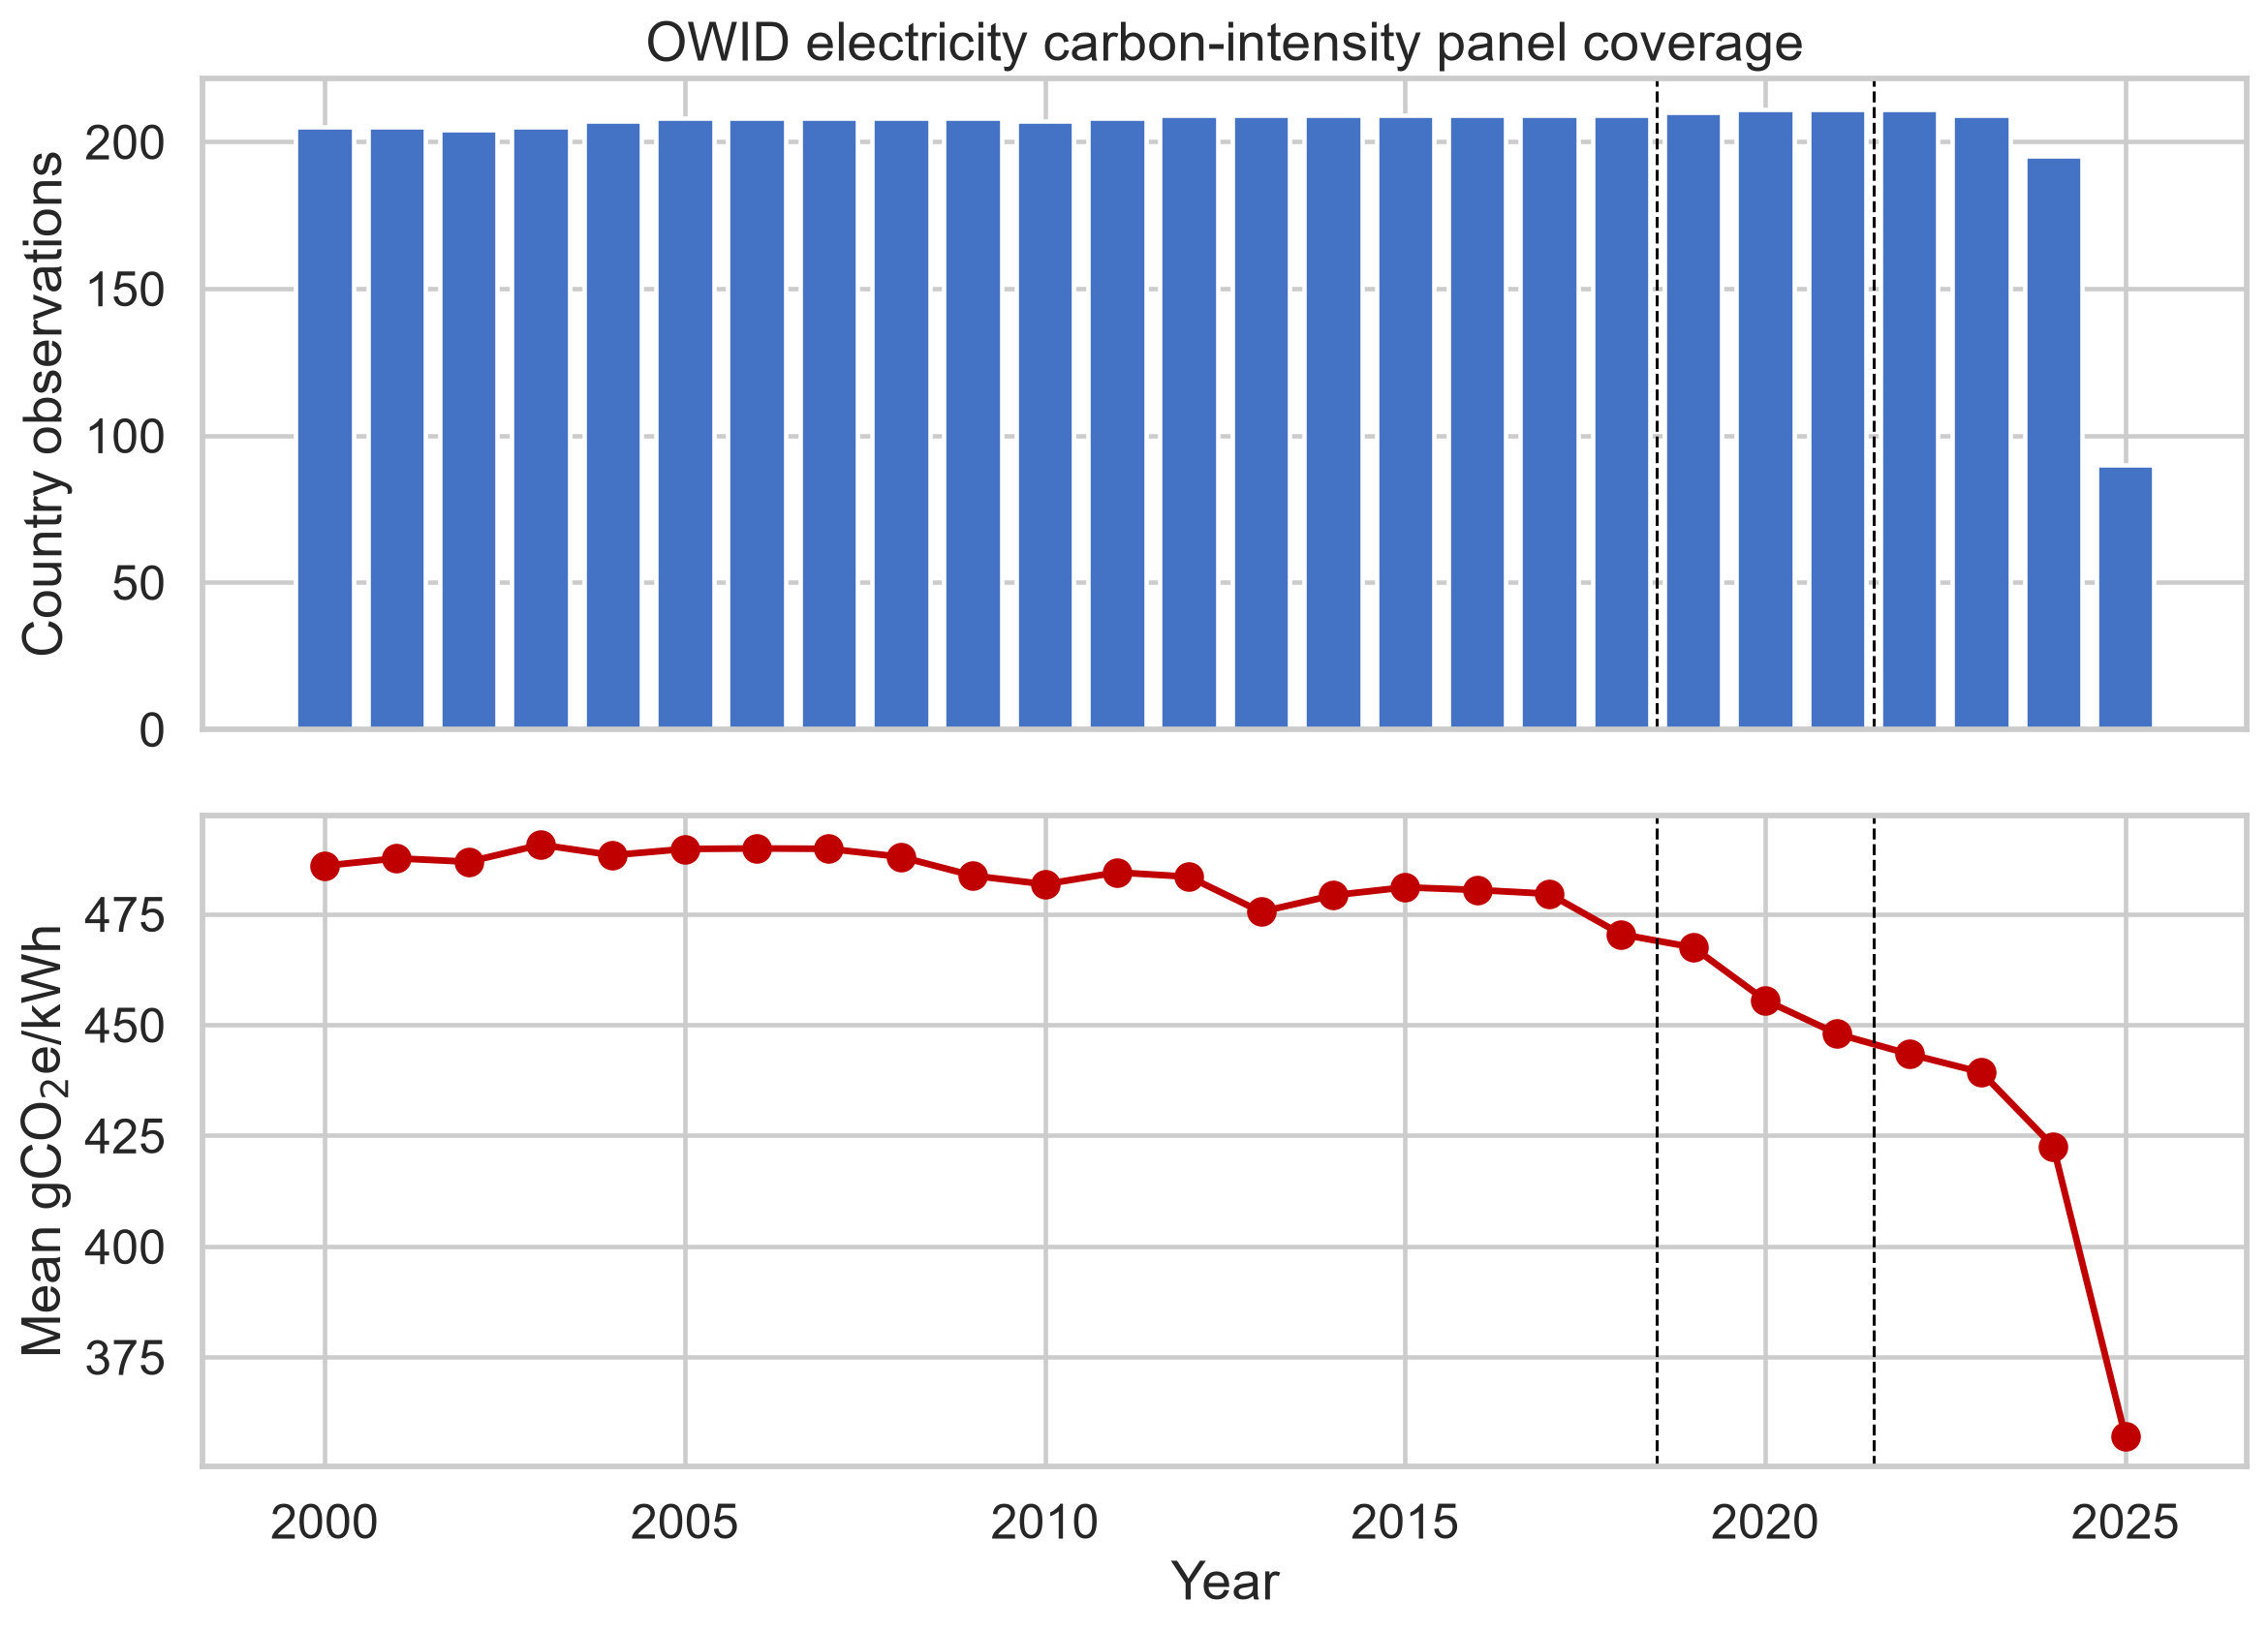
\includegraphics[width=0.76\linewidth]{../../outputs/carbon_intensity/figures/dataset_coverage_and_trend.png}
  \caption{Độ phủ dữ liệu và cường độ carbon trung bình theo năm.}
  \label{fig:coverage}
\end{figure}

\subsection{So sánh mô hình}

Bảng~\ref{tab:metrics} được sinh trực tiếp từ
\texttt{model\_metrics.csv}. Trên test 2022--2025, \BestModel{} có sai số thấp
nhất với MAE \BestTestMAE{}, RMSE \BestTestRMSE{} gCO$_2$e/kWh và
$R^2=\BestTestRSquared$. Kết quả validation và test có cùng thứ hạng mô hình,
giảm nguy cơ kết luận chỉ dựa trên một tập duy nhất.

\begin{table}[H]
  \centering
  \caption{Kết quả validation và temporal test.}
  \label{tab:metrics}
  \resizebox{\textwidth}{!}{% Auto-generated experimental metrics.
\begin{tabular}{llrrrr}
\toprule
Tập dữ liệu & Mô hình & $n$ & MAE & RMSE & $R^2$ \\
\midrule
Test (2022-2025) & XGBoost & 705 & 24.25 & 41.03 & 0.972 \\
Test (2022-2025) & Random Forest & 705 & 29.77 & 47.14 & 0.962 \\
Test (2022-2025) & Linear Regression & 705 & 43.54 & 77.83 & 0.898 \\
Validation (2019-2021) & XGBoost & 632 & 25.82 & 48.24 & 0.961 \\
Validation (2019-2021) & Random Forest & 632 & 29.97 & 48.78 & 0.960 \\
Validation (2019-2021) & Linear Regression & 632 & 43.60 & 81.83 & 0.887 \\
\bottomrule
\end{tabular}
}
\end{table}

\begin{figure}[H]
  \centering
  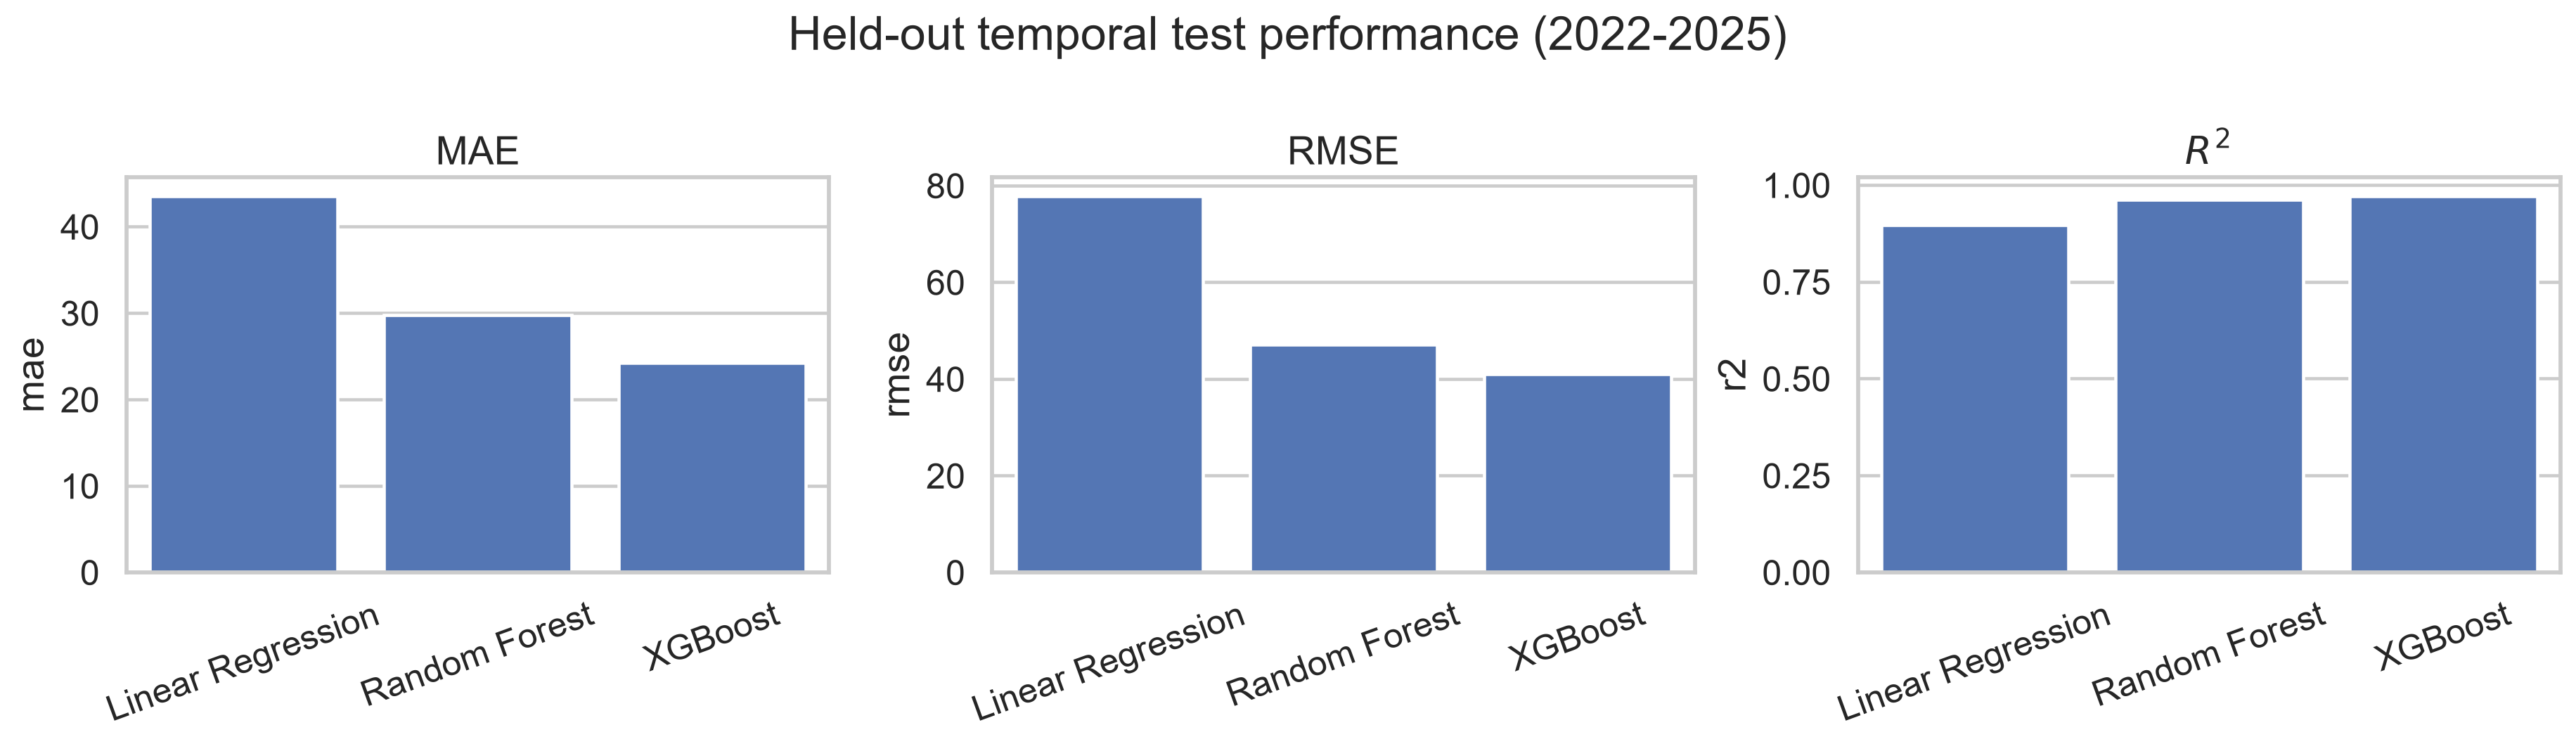
\includegraphics[width=\linewidth]{../../outputs/carbon_intensity/figures/model_comparison_test.png}
  \caption{So sánh MAE, RMSE và $R^2$ trên test 2022--2025.}
  \label{fig:comparison}
\end{figure}

Hình~\ref{fig:actual} cho thấy dự đoán của mô hình tốt nhất bám gần đường
$y=\hat{y}$ trên phần lớn miền giá trị. Hình~\ref{fig:residual} cho thấy phân bố
phần dư theo từng năm test; độ phân tán lớn hơn ở một số năm nhấn mạnh lợi ích
của báo cáo sai số theo thời gian thay vì chỉ một số tổng hợp.

\begin{figure}[H]
  \centering
  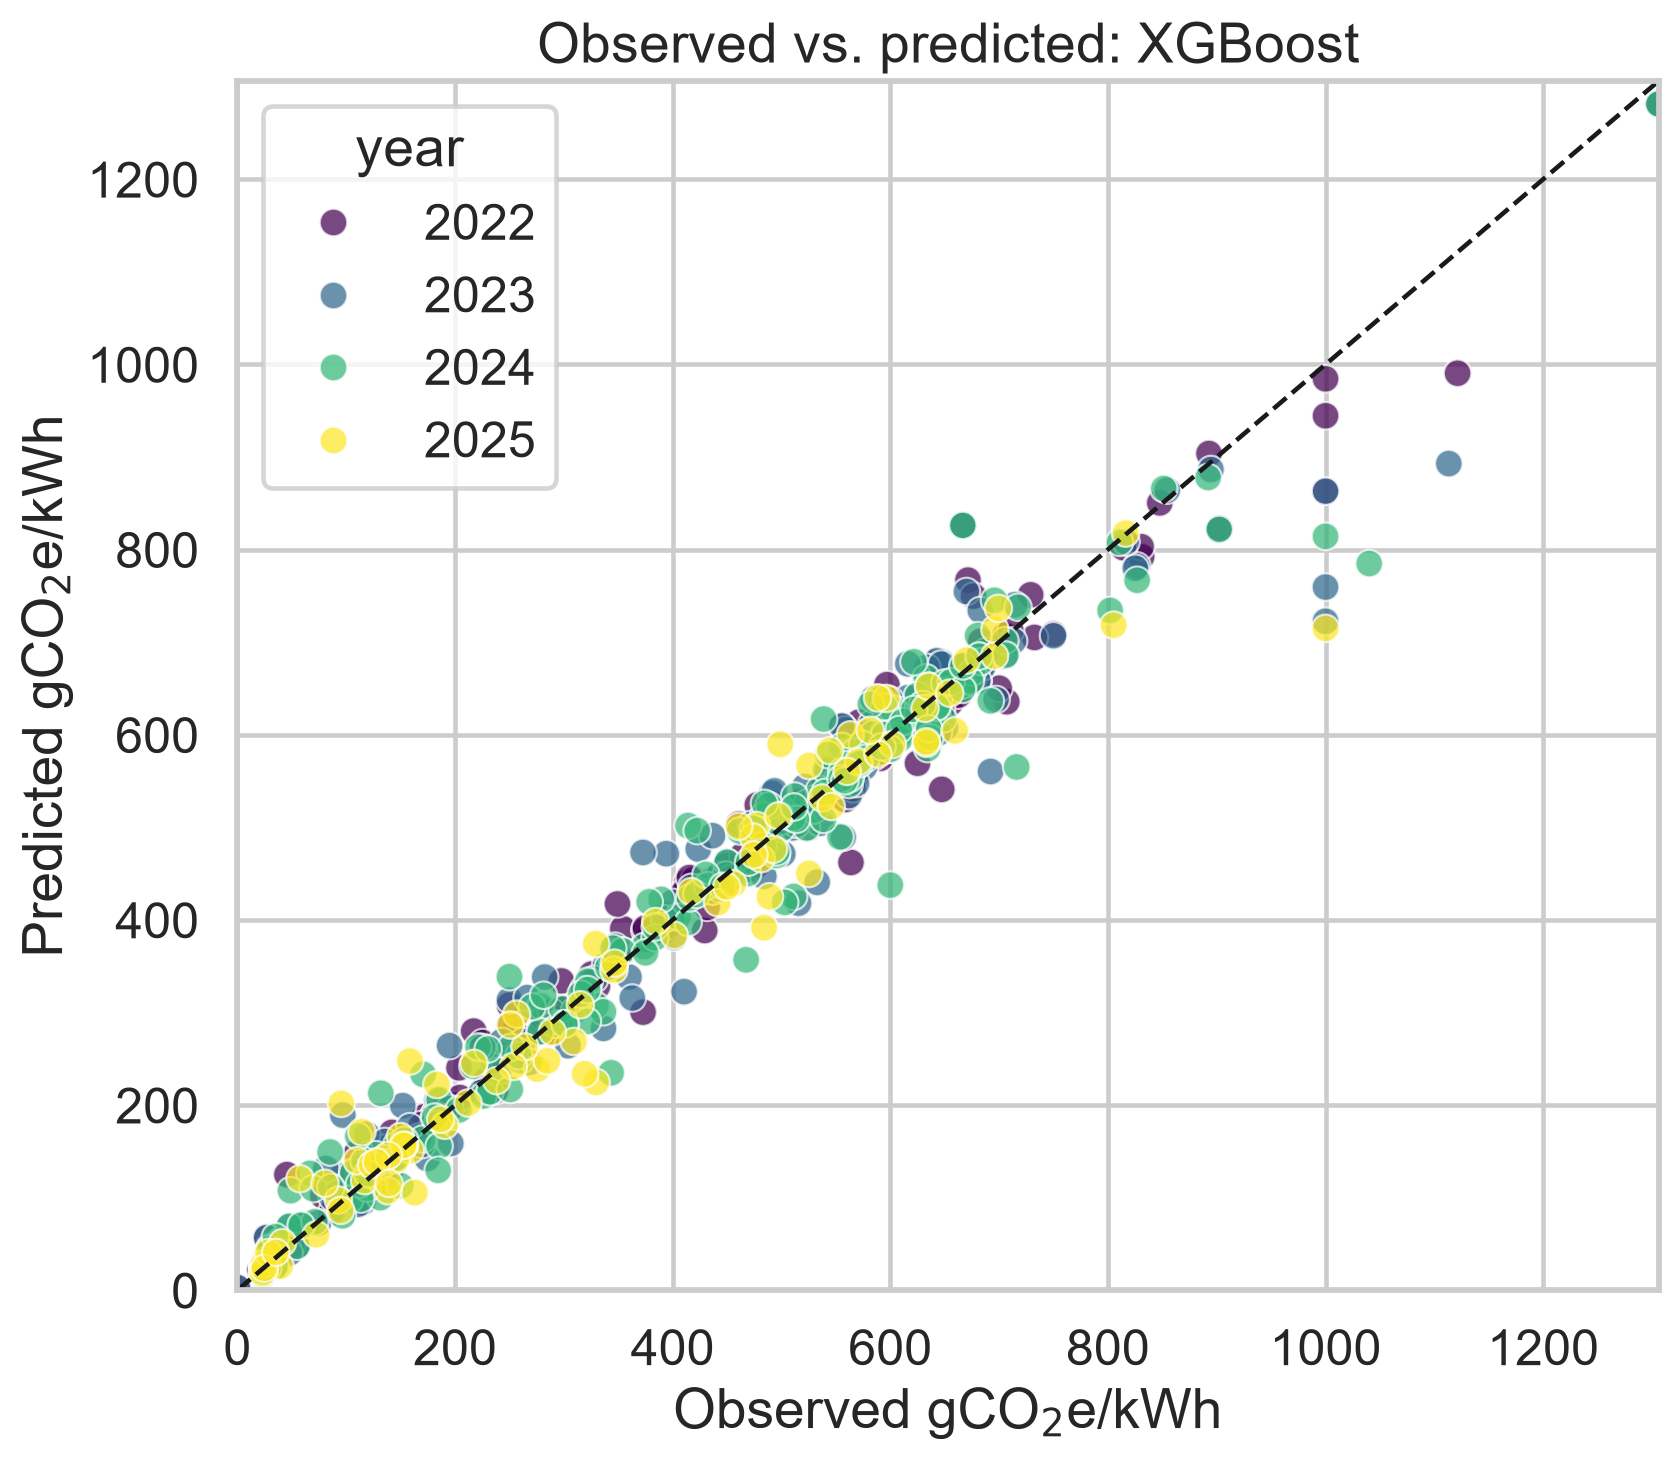
\includegraphics[width=0.76\linewidth]{../../outputs/carbon_intensity/figures/actual_vs_predicted_best.png}
  \caption{Giá trị quan sát và dự đoán của mô hình tốt nhất trên tập test.}
  \label{fig:actual}
\end{figure}

\begin{figure}[H]
  \centering
  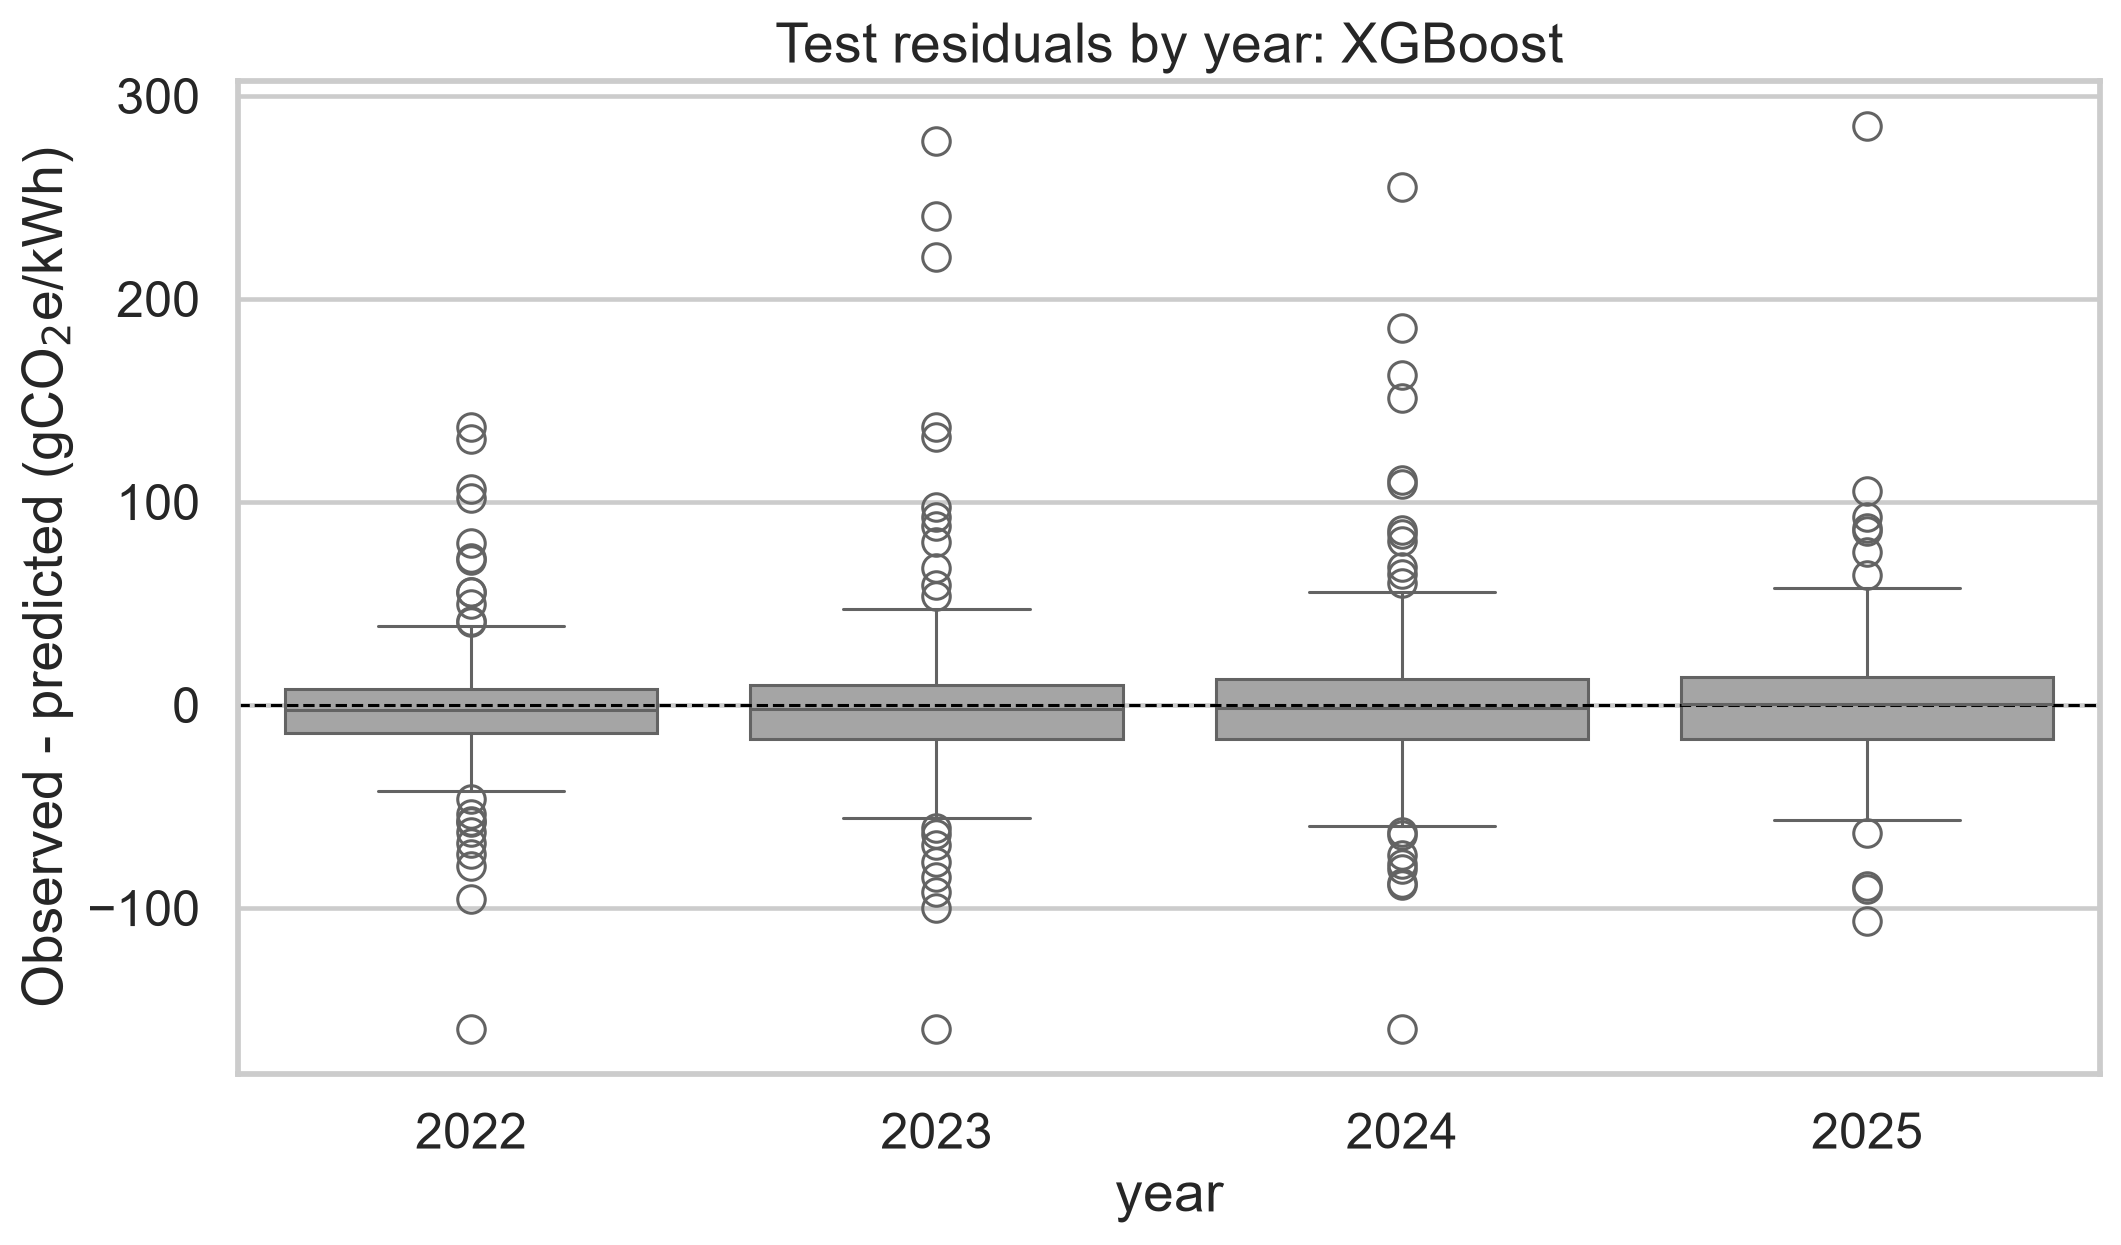
\includegraphics[width=0.82\linewidth]{../../outputs/carbon_intensity/figures/residuals_by_year_best.png}
  \caption{Phần dư test theo năm của mô hình tốt nhất.}
  \label{fig:residual}
\end{figure}

\subsection{Feature importance và SHAP}

Importance nội tại của Random Forest và XGBoost được trình bày ở
Hình~\ref{fig:importance}. Vì importance dựa trên cách chia cây có thể ưu tiên
một trong các biến tương quan, nghiên cứu bổ sung permutation importance và
SHAP. Trên mẫu tối đa 500 hàng test cố định bằng seed 42,
\TopSHAPFeature{} có mean absolute SHAP lớn nhất (Bảng~\ref{tab:shap}).

\begin{figure}[H]
  \centering
  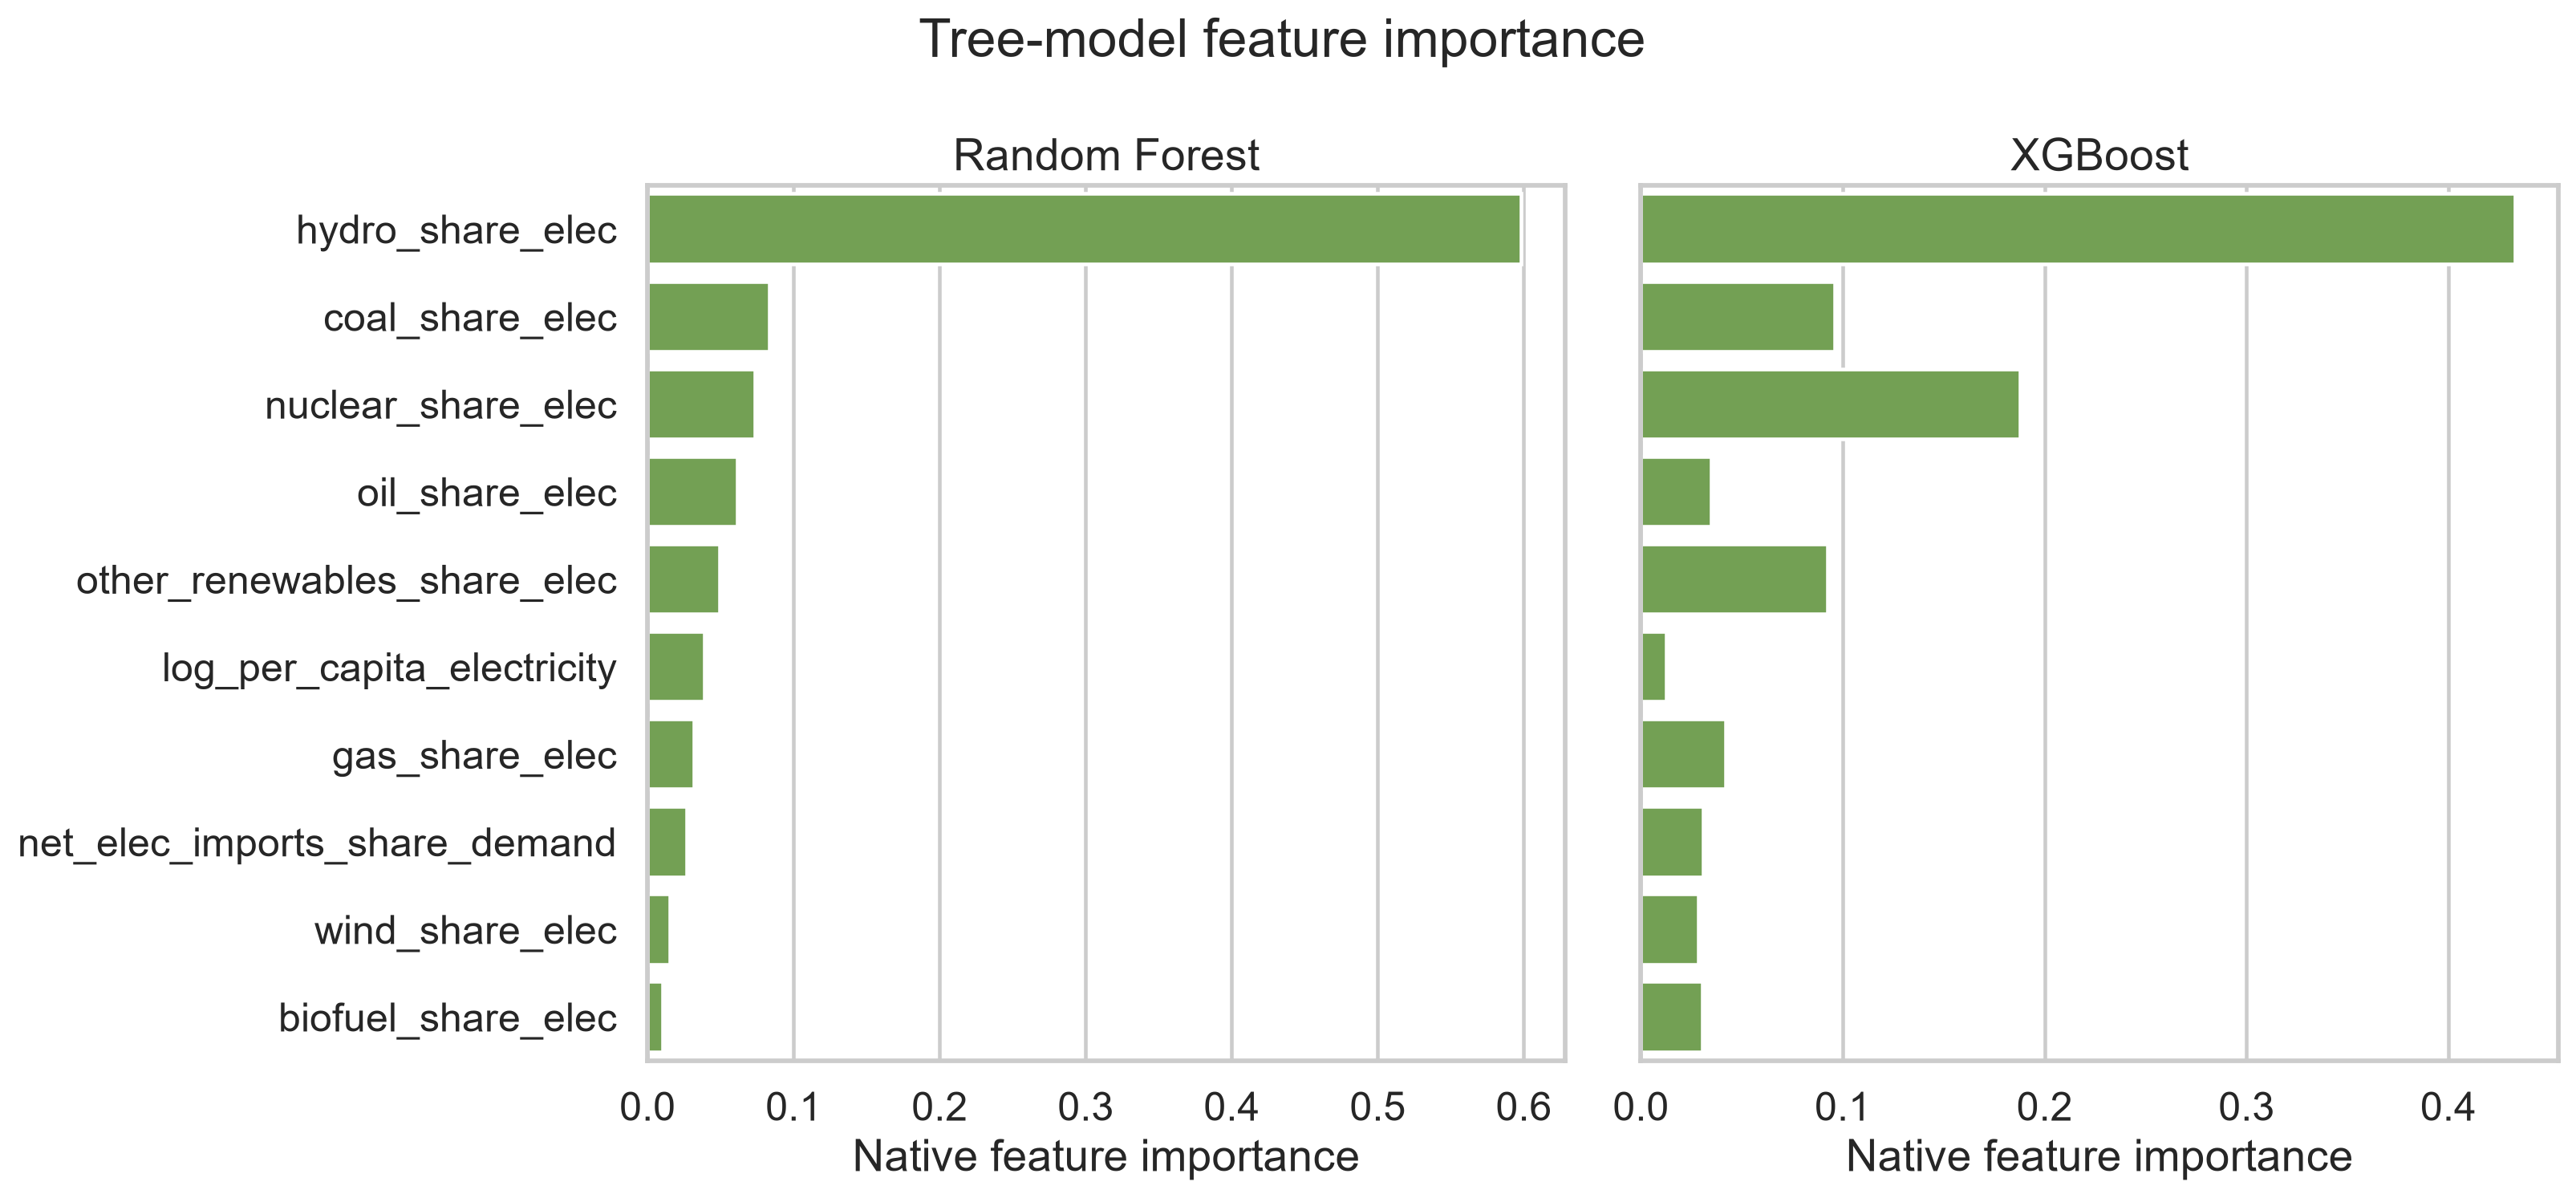
\includegraphics[width=\linewidth]{../../outputs/carbon_intensity/figures/tree_feature_importance.png}
  \caption{Feature importance nội tại của hai mô hình cây.}
  \label{fig:importance}
\end{figure}

\begin{table}[H]
  \centering
  \caption{Tám đặc trưng có mean absolute SHAP cao nhất của XGBoost.}
  \label{tab:shap}
  % Auto-generated SHAP ranking.
\begin{tabular}{lr}
\toprule
Đặc trưng & Mean $|$SHAP$|$ \\
\midrule
\texttt{hydro\_share\_elec} & 123.47 \\
\texttt{coal\_share\_elec} & 51.05 \\
\texttt{oil\_share\_elec} & 27.05 \\
\texttt{gas\_share\_elec} & 25.85 \\
\texttt{nuclear\_share\_elec} & 24.85 \\
\texttt{solar\_share\_elec} & 24.21 \\
\texttt{other\_renewables\_share\_elec} & 23.10 \\
\texttt{wind\_share\_elec} & 22.43 \\
\bottomrule
\end{tabular}

\end{table}

\begin{figure}[H]
  \centering
  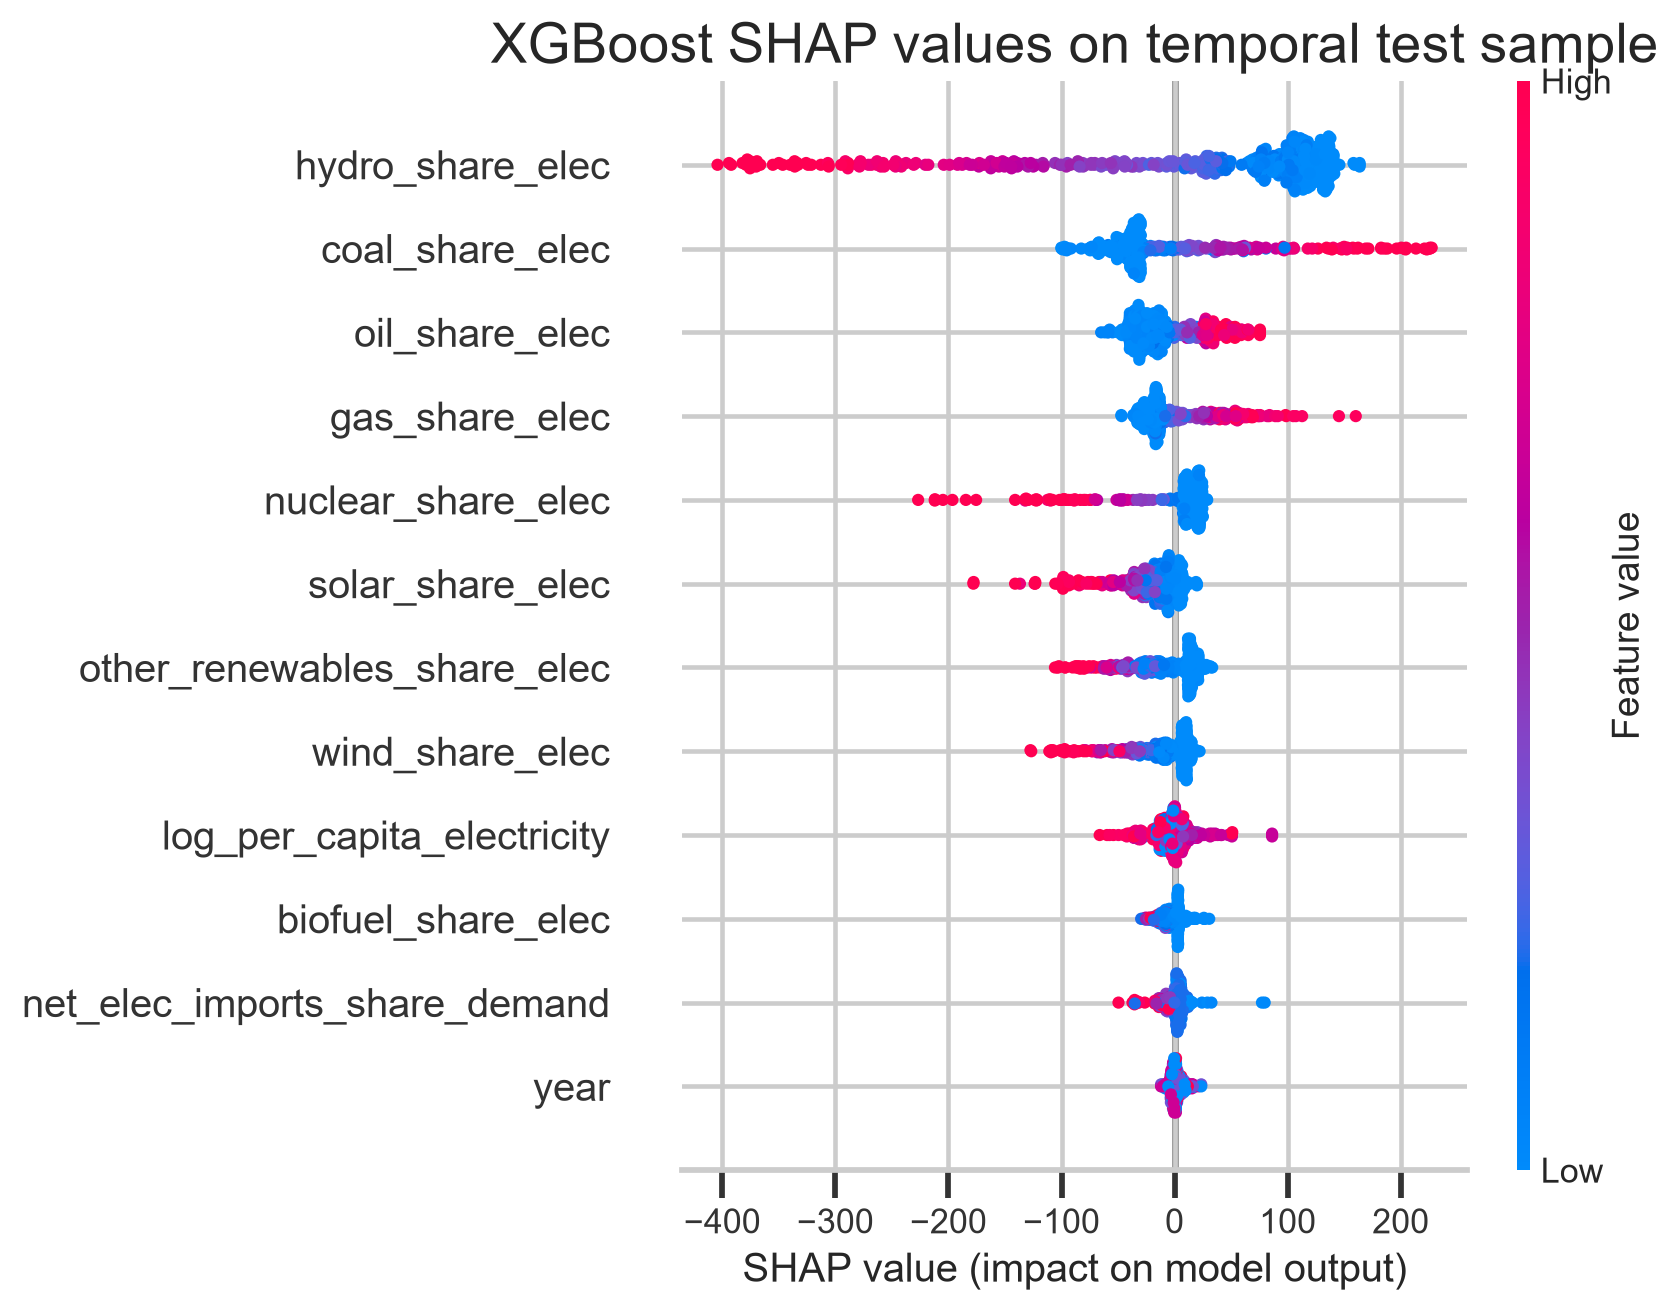
\includegraphics[width=0.88\linewidth]{../../outputs/carbon_intensity/figures/xgboost_shap_beeswarm.png}
  \caption{Phân bố SHAP của XGBoost trên mẫu test. Màu biểu diễn giá trị đặc trưng.}
  \label{fig:shap}
\end{figure}

\section{Thảo luận}

XGBoost vượt Random Forest và Linear Regression trên cả validation lẫn test,
cho thấy các quan hệ phi tuyến và tương tác giữa các thành phần cơ cấu điện mang
thông tin dự báo đáng kể. Linear Regression vẫn đạt $R^2$ dương cao nhưng có
RMSE lớn hơn, phù hợp với vai trò baseline. Các tỷ trọng nguồn điện chi phối
SHAP là hợp lý về mặt cấu trúc vì biến đích phản ánh tổng hợp phát thải vòng đời
của hỗn hợp phát điện. Tuy nhiên, một thứ hạng SHAP cao không có nghĩa tăng một
điểm phần trăm của nguồn đó sẽ gây ra đúng mức thay đổi tương ứng: quan hệ cấu
thành, nhập khẩu và các biến bị bỏ sót làm giới hạn diễn giải can thiệp.

Kết quả nên được dùng cho kiểm tra nhất quán dữ liệu, ước lượng giá trị thiếu hoặc
nowcasting khi cơ cấu điện cùng năm đã biết. Để dự báo thực sự cho các năm chưa
có cơ cấu điện, cần xây dựng biến trễ hoặc kịch bản ngoại sinh cho tỷ trọng nguồn,
nhu cầu, chính sách và công suất lắp đặt; đó là bài toán khác với phạm vi hiện tại.

\section{Giới hạn và nguy cơ đối với độ tin cậy}

\begin{itemize}
  \item \textbf{Độ phủ 2025:} chỉ một phần quốc gia có quan sát 2025. Metric gộp
  test vì vậy chịu ảnh hưởng của cấu thành mẫu và không đại diện hoàn toàn cho
  mọi quốc gia.
  \item \textbf{Phụ thuộc panel:} cùng quốc gia xuất hiện ở nhiều năm. Temporal
  split ngăn leakage theo năm nhưng không đo khả năng tổng quát sang quốc gia
  hoàn toàn chưa thấy.
  \item \textbf{Nowcasting thay vì dự báo dài hạn:} đặc trưng và biến đích cùng
  năm. Kết quả không chứng minh mô hình biết trước cơ cấu điện tương lai.
  \item \textbf{Dữ liệu quan sát:} sai số đo, cập nhật hồi tố và khác biệt phương
  pháp nguồn có thể truyền vào mô hình.
  \item \textbf{Diễn giải:} native importance, permutation importance và SHAP
  mô tả hành vi mô hình, không phải ước lượng nhân quả.
  \item \textbf{Tái lập theo thời gian:} OWID cập nhật thường xuyên; checksum của
  snapshot là điều kiện để tái tạo đúng các số liệu trong bài.
\end{itemize}

\section{Khả năng tái lập}

Notebook chính trong thư mục \texttt{notebooks} chạy toàn bộ quy trình từ kiểm
tra nguồn tới mô hình và SHAP. Mã dùng chung nằm
trong \path{src/carbon_intensity_workflow.py}. Seed, phiên bản thư viện,
danh sách đặc trưng và split được ghi vào \path{environment.json}. Prediction
test, metric tổng hợp, metric theo năm, lưới siêu tham số, importance, mô hình
đã fit và hình đều được lưu dưới \path{outputs/carbon_intensity/}. Các macro
và bảng trong paper được sinh từ CSV thực nghiệm, không nhập thủ công.

\section{Kết luận}

Nghiên cứu đã triển khai một workflow có provenance và chia dữ liệu theo thời
gian để ước lượng cường độ carbon điện từ OWID/Ember giai đoạn 2000--2025.
Trong ba mô hình, \BestModel{} đạt kết quả test tốt nhất với MAE
\BestTestMAE{}, RMSE \BestTestRMSE{} gCO$_2$e/kWh và
$R^2=\BestTestRSquared$. Kết quả hỗ trợ sử dụng mô hình cây tăng cường cho bài
toán dữ liệu bảng này, đồng thời nhấn mạnh rằng hiệu năng cao không loại bỏ giới
hạn về độ phủ 2025, phụ thuộc theo quốc gia và diễn giải nhân quả. Bước tiếp theo
hợp lý là đánh giá leave-country-out, mô hình dùng biến trễ, và các kịch bản cơ
cấu nguồn điện tương lai.

\section*{Dữ liệu và mã nguồn}

Dữ liệu OWID được sử dụng theo điều kiện ghi công của nguồn. URL, thời điểm tệp,
kích thước và SHA-256 được lưu trong artifact provenance. Mã, notebook và kết
quả thực nghiệm đi kèm paper trong cùng repository.

\begin{thebibliography}{9}

\bibitem{owid-carbon-intensity}
H. Ritchie, P. Rosado, and M. Roser,
``Lifecycle carbon intensity of electricity generation,''
\emph{Our World in Data}, data adapted from Ember, 2026.
\url{https://ourworldindata.org/grapher/carbon-intensity-electricity}.

\bibitem{owid-energy-data}
Our World in Data,
``Data on Energy by Our World in Data,'' 2026.
\url{https://github.com/owid/energy-data}.

\bibitem{ember-methodology}
Ember,
``Yearly Electricity Data: Methodology,'' 2026.
\url{https://files.ember-energy.org/public-downloads/ember_electricity_data_methodology.pdf}.

\bibitem{breiman2001}
L. Breiman,
``Random Forests,'' \emph{Machine Learning}, vol. 45, pp. 5--32, 2001.
doi: \href{https://doi.org/10.1023/A:1010933404324}{10.1023/A:1010933404324}.

\bibitem{chen2016}
T. Chen and C. Guestrin,
``XGBoost: A Scalable Tree Boosting System,'' in \emph{Proceedings of the 22nd
ACM SIGKDD International Conference on Knowledge Discovery and Data Mining},
pp. 785--794, 2016.
doi: \href{https://doi.org/10.1145/2939672.2939785}{10.1145/2939672.2939785}.

\bibitem{lundberg2017}
S. M. Lundberg and S.-I. Lee,
``A Unified Approach to Interpreting Model Predictions,'' in
\emph{Advances in Neural Information Processing Systems 30}, 2017.
\url{https://proceedings.neurips.cc/paper/7062-a-unified-approach-to-interpreting-model-predictions}.

\end{thebibliography}

\end{document}
